\documentclass[a4paper,14pt]{extreport}
\usepackage[left=1.5cm,right=1.5cm,
    top=1.5cm,bottom=2cm,bindingoffset=0cm]{geometry}
\usepackage{scrextend}
\usepackage[T1,T2A]{fontenc}
\usepackage[utf8]{inputenc}
\usepackage[english,russian,ukrainian]{babel}
\usepackage{tabularx}
\usepackage{amssymb}
\usepackage{color}
\usepackage{amsmath}
\usepackage{mathrsfs}
\usepackage{listings}
\usepackage{graphicx}
\graphicspath{ {./images/} }
\usepackage{lipsum}
\usepackage{xcolor}
\usepackage{hyperref}
\usepackage{tcolorbox}
\usepackage{tikz}
\usepackage[framemethod=TikZ]{mdframed}
\usepackage{wrapfig,boxedminipage,lipsum}
\mdfdefinestyle{MyFrame}{%
linecolor=blue,outerlinewidth=2pt,roundcorner=20pt,innertopmargin=\baselineskip,innerbottommargin=\baselineskip,innerrightmargin=20pt,innerleftmargin=20pt,backgroundcolor=gray!50!white}
 \usepackage{csvsimple}
 \usepackage{supertabular}
\usepackage{pdflscape}
\usepackage{fancyvrb}
%\usepackage{comment}
\usepackage{array,tabularx}
\usepackage{colortbl}

\usepackage{varwidth}
\tcbuselibrary{skins}
\usepackage{fancybox}


\usepackage{tikz}
\usepackage[framemethod=TikZ]{mdframed}
\usepackage{xcolor}
\usetikzlibrary{calc}
\makeatletter
\newlength{\mylength}
\xdef\CircleFactor{1.1}
\setlength\mylength{\dimexpr\f@size pt}
\newsavebox{\mybox}
\newcommand*\circled[2][draw=blue]{\savebox\mybox{\vbox{\vphantom{WL1/}#1}}\setlength\mylength{\dimexpr\CircleFactor\dimexpr\ht\mybox+\dp\mybox\relax\relax}\tikzset{mystyle/.style={circle,#1,minimum height={\mylength}}}
\tikz[baseline=(char.base)]
\node[mystyle] (char) {#2};}
\makeatother

\definecolor{ggreen}{rgb}{0.4,1,0}
\definecolor{rred}{rgb}{1,0.1,0.1}
\definecolor{amber}{rgb}{1.0, 0.75, 0.0}
\definecolor{babyblue}{rgb}{0.54, 0.81, 0.94}
\definecolor{asparagus}{rgb}{0.53, 0.66, 0.42}
\definecolor{chartreuse}{rgb}{0.5, 1.0, 0.0}
\definecolor{darkorchid}{rgb}{0.6, 0.2, 0.8}

\usepackage{float}
\usepackage{wrapfig}
\usepackage{framed}
%for nice Code{
\lstdefinestyle{customc}{
  belowcaptionskip=1\baselineskip,
  breaklines=true,
  frame=L,
  xleftmargin=\parindent,
  language=C,
  showstringspaces=false,
  basicstyle=\small\ttfamily,
  keywordstyle=\bfseries\color{green!40!black},
  commentstyle=\itshape\color{purple!40!black},
  identifierstyle=\color{blue},
  stringstyle=\color{orange},
}
\lstset{escapechar=@,style=customc}
%}


\begin{document}
\pagecolor{white}

%----------------------------------------1
\newtcbox{\xmybox}[1][red]{on line, arc=7pt,colback=#1!10!white,colframe=#1!50!black, before upper={\rule[3pt] {0pt}{10pt}},boxrule=1pt,boxsep=0pt,left=6pt,right=6pt,top=2pt,bottom=2pt}

\begin{center}\xmybox[green]{Mnatsakanov Anton} \xmybox[amber]{DP-82} \xmybox[blue]{Variant №5}
\vspace{1cm}

\end{center}


\begin{center}В яких діелектриках спостерігається п’єзоелектричний ефект? Поясність геометрично (на рисунках) різницю прямого і оберненого п’єзоефекту.\end{center}

At the moment, the industry of practical applications of devices and appliances that use the piezo effect in their constructions is constantly expanding. Some products such as watches, cameras, cell phones, televisions, computers and piezo lighters have become everyday items. It is difficult to even list the various electronic devices that are impossible without the use of piezo elements. They are emitters and antennas in hydroacoustics, frequency stabilizers in computers, radio devices and time standards, electrical filters and delay lines in radio and telephone communications, sensors for measuring acceleration, vibration level, acoustic emission for nondestructive testing, p  ezotransformers and ultrasonic motor, medical ultrasonic tomography and medical instruments for various purposes and so on.\par
Piezoelectric materials include bulk ceramics, ceramic thin films, multilayer ceramics, single crystals, polymers and ceramic-polymer composites. In recent years, a large number of different piezoelectric film materials have been developed and tested for use in various microsystems and microelectronic components. It has been found that film and bulk piezoelectric elements are advantageous for ultrahigh-frequency devices. New relaxor-selectric ceramics and crystals exhibit extremely high piezoelectric energy conversion efficiency, of interest, in particular, for medical imaging devices and for other applications, such as special drives for industrial non-destructive testing.\par
Various electromechanical effects occur in dielectrics in an electric field: "free" crystal deforms under the action of the field, and mechanical stresses arise in the "clamped" crystal. The physical cause of such electromechanical effects is microscopic shifts of electric charges under the influence of the applied electric field: electric polarization is necessarily accompanied by mechanical effects. The nature of the dependence of electrically induced mechanical deformation on the electric field strength is determined by the symmetry of the dielectric structure.\par
In dielectrics with a centrosymmetric structure, the sign of the deformation induced by the electric field does not depend on the electric polarity of the applied field E (the effect is quadratic, that is, the field-induced deformation x is proportional to E2). This effect, called electrostriction, is characteristic of all dielectrics without exception. Usually there is mechanical stretching in the direction of the applied field and compression in the direction perpendicular to the field. So, a centrosymmetric dielectric partially converts electrical energy into mechanical energy (but not vice versa). For most dielectrics the electrostriction effect is very small, but at the moment such dielectrics (segmentelectric relaxors with a blurred phase transition) have been found in which giant electrostriction is observed, which is used in technical devices.\par
In dielectrics with a noncentrosymmetric structure, in addition to electrostriction, there is another electromechanical effect: piezoelectric. It can be assumed that the cause of this effect is the dielectric's own (internal) electric moment, caused in noncentrosymmetric structures by the electric interaction of the electron shells of ions or molecules and their spontaneous deformation (in the absence of external influence). In the case of an externally applied electric field, the deformation is linear in field: the sign of the mechanical strain x induced by the field is reversed if the electric polarity E changes. Moreover, the piezoelectric effect, unlike electrostriction, is reversed: in those dielectrics in which it occurs, the externally applied mechanical stress, in turn, causes electric polarization.\par
So, a piezoelectric is capable of transforming mechanical energy into electrical energy, or, conversely, electrical energy into mechanical energy. At first, the first of these effects was observed, which is why it is called the "direct" piezoelectric effect.
The direct piezoelectric effect consists in the fact that under the action of mechanical stress X, or elastic deformation x caused by mechanical stress, electrical polarization occurs in noncentrosymmetric dielectrics (piezoelectricity) (Fig. 1, a, b, c).\par
Since the electrical conductivity of the piezoelectric (dielectric) is very small, the polarization is manifested in the form of mechanically induced electric charges that occur on the surface of the deformed piezoelectric. The density of these charges is described by the piezo-induced polarization P, and the direction of the polarization vector is chosen from the mark - to the mark + , as shown in Fig. 1, b, c. The polarization is proportional to the electrical induction D.
If there are no external mechanical influences (X = 0, x = 0), then free charges do not occur on the surface of the piezoelectric and therefore the piezoelectric is not polarized (Fig. 1, a). It becomes polarized as a result of "positive" tensile deformation (x> 0) or "negative" compression deformation (x <0). Changing the sign of mechanical impact, for example, when the compression (Fig. 1, b) is replaced by stretching (Fig. 1, c), causes a change in the sign of electrical polarization R. In the case of a direct piezoelectric effect, the polarization value is directly proportional to the deformation:



\begin{figure}[h]
\center{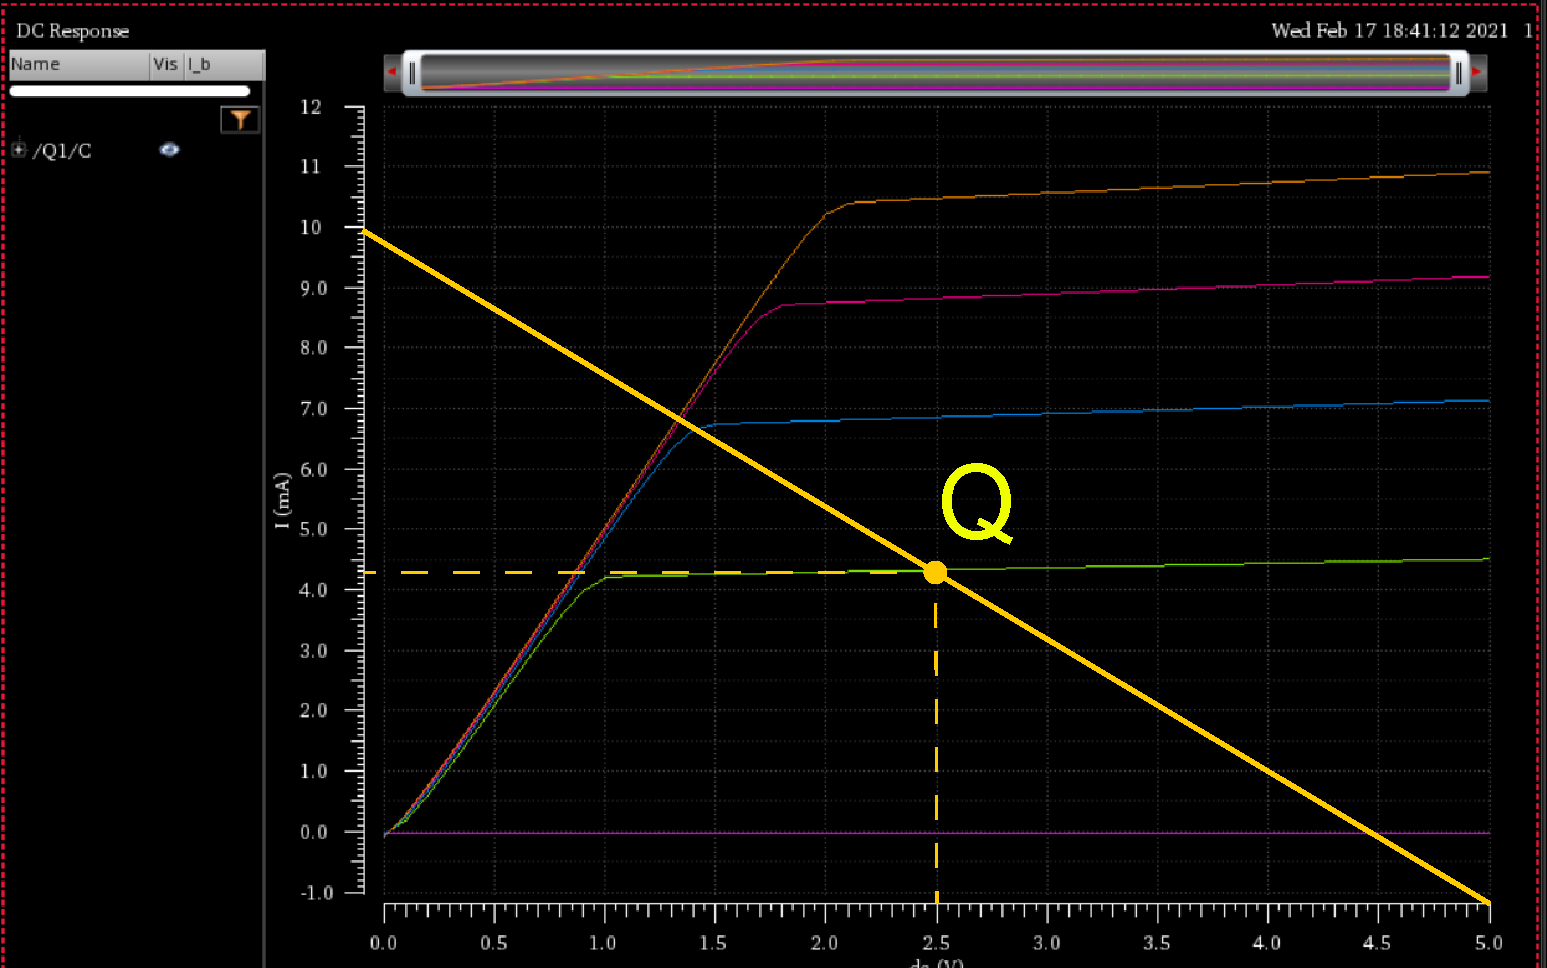
\includegraphics[width=0.6\linewidth]{1.png}}
\caption{Explanation of direct (b, c, f) and inverse (d, e, i) piezoelectric effects.}
\label{ris1}
\end{figure}
\end{document}
